%% A chapter for my PhD dissertation
%% First author: Theodore Pak
%%
%% Must be included from main.tex.

\chapter{Estimating local costs of \emph{Clostridium difficile} infection using statistical learning and electronic medical records}
\label{chap:cdi_cost}

\begin{quote}
\emph{Reported per-patient costs of \emph{Clostridium difficile} infection (CDI) vary by two orders of magnitude among different hospitals, suggesting that precise, local analyses are needed to guide decision-making. We sought to estimate changes in length of stay (LOS) associated with CDI at one hospital using only automatically extractable electronic medical record (EMR) data and performed a retrospective cohort study of 171,938 visit records spanning a 7-year period. 23,968 variables were extracted from EMR data recorded within 24 hours of each admission to train an elastic net regularized logistic regression model for propensity score matching. To address time-dependent bias (reverse causation), we stratified comparisons by time-of-infection and fit multistate models. The estimated difference in median LOS for propensity-matched cohorts varied from 3.1 days (95\% CI, 2.2–3.9) to 10.1 days (95\% CI, 7.3–12.2) depending on the case definition; however, dependency of the estimate on time-to-infection was observed. Stratification by time to first positive toxin assay, excluding probable community-acquired infections, showed a minimum excess LOS of 3.1 days (95\% CI, 1.7–4.4). Under the same case definition, the multistate model averaged an excess LOS of 3.3 days (95\% CI, 2.6–4.0). Changes in LOS can be extrapolated to a marginal dollar cost per CDI case by multiplying by the average cost of an inpatient-day. We conclude that infection control officers can leverage automatically extractable EMR data to estimate costs of CDI at their specific institution.
}
\end{quote}

\newthought{\emph{Clostridium difficile} infection} (CDI) is the most frequently reported healthcare-associated infection (HAI) in the US\sidecite[-2cm]{Leffler2015} and the major infective cause of nosocomial diarrhea in developed countries,\sidecite[-1.9cm]{Davies2014} incurring billions of dollars in excess medical costs per year.\autocite{Zimlichman2013} Estimates of the per-patient cost of CDI have varied from \$2,871 to \$122,318 due to differences in methodology, patient inclusion criteria, and regional costs.\autocite{Gabriel2014,Ghantoji2010,Zhang2016} Given the high hospital-to-hospital variability of these costs,\autocite{Lofgren2014,Stevens2015} infection control officers, hospital administrators, and clinicians would benefit from estimates tailored to their particular population and healthcare practices. Concretely defining the potential economic savings of CDI prevention would empower stakeholders to prudently choose among the many available validated interventions.\autocite{Dubberke2014a,Katz2013}

Measuring costs within healthcare systems is notoriously difficult (particularly in the US), as many hospitals do not have access to structured, itemized reimbursement data linked to all of their patient medical records.\autocite{Cooper2015} Even the institutions that have informatics capabilities to retrospectively link these data have relied on the curation of select variables and chart review to estimate attributable CDI cost.\autocite{Dubberke2008,Dubberke2014,Greco2015} Nevertheless, electronic medical record (EMR) systems are used by the majority of first-world acute care facilities.\autocite{Gray2011,Henry2016} Part of the rationale for these systems is that hospitals may leverage EMR data for optimal decision-making by inferring causal relationships from raw observations during routine care.\autocite{Dahabreh2014,Etheredge2007,Pak2015} An analysis based on automatically extractable data from an EMR that quantifies preventable hospital costs, such as those attributable to an HAI like CDI, would be of great value in building a continuously learning healthcare system.\autocite{Krumholz2016} EMRs contain many structured fields relevant to this analysis, including: diagnosis codes and lab results demonstrating onset of HAIs; thousands of variables for procedures, problems, and medications that can serve as covariates for adjustment in observational studies; and importantly, the length of stay (LOS) for each visit, which is the primary contributor to excess costs for most HAIs, including CDI.\autocite{McGlone2012,Wilcox1996,Zimlichman2013}

The goal of this study was to generate a robust estimate of local cost associated with CDI using data that are automatically extractable from a typical EMR. We use all available structured data recorded within 24 hours of admission in the EMR—including over 20,000 variables, such as medications reported and administered, abnormal lab values, and problem list entries—to build fully data-driven models for CDI risk using a machine learning algorithm, avoiding the potential bias of preselected covariates and manual chart review. CDI risk models trained on uncurated data from EMRs have already outperformed models that only incorporate variables for known risk factors, indicating that CDI risk may be nuanced in particular care settings.\autocite{Wiens2014} We then use these trained CDI risk models for propensity score matching, which allows estimation of changes in LOS associated with CDI. Most previous studies of CDI cost do not account for the possibility that longer LOS increases the risk of CDI, i.e., reverse causation, and therefore likely overestimate the cost of CDI.\autocite{Mitchell2014,Stevens2015} To adjust for this, we stratify our analysis by the time of CDI diagnosis to find the change in LOS conditional on minimal prior exposure to the hospital environment. Finally, we compare these results to a multistate model of competing time-dependent risks between discharge and the onset of CDI.

\section{Methods}

\subsection{Data source}

\begin{figure}[htb]
  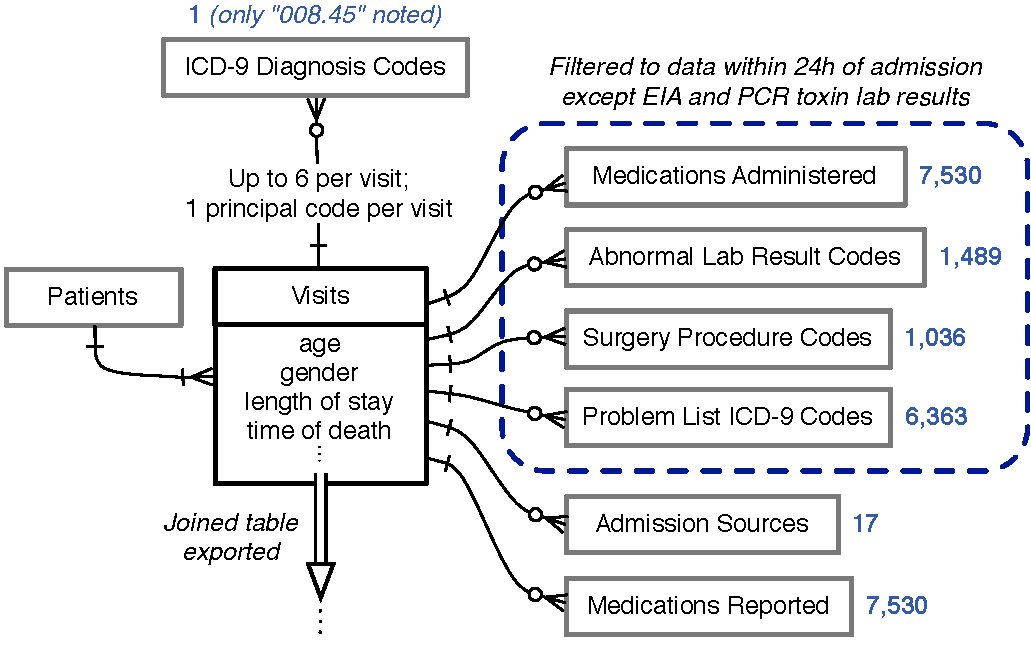
\includegraphics[width=\textwidth]{chap5/1a_methods_db_schema}               
  \caption[Data sources for this study]{\textbf{Data sources for this study}. Entity-relationship diagram for all electronic medical record data used to generate models of \emph{Clostridium difficile} infection propensity, using Information Engineering notation; see \textcite{Halpin2010}. Boxes represent tables of entities with any directly associated attributes (fields) listed below; single lines represent relationships, with arrowheads indicating the cardinality of each side of the relationship; crow’s foot arrowhead with circle represents “zero or more;” crow’s foot arrowhead with cross-stroke represents “one or more;” cross-stroke arrowhead represents “exactly one.” Blue numbers indicate the number of variables extracted from each associated table for each visit. ICD-9, International Classification of Diseases Ninth Revision; EIA, enzyme immunoassay; PCR, polymerase chain reaction.}
  \label{fig:db_schema}
\end{figure}

This study was conducted at The Mount Sinai Hospital, a 1,171-bed tertiary care hospital in New York, NY. Records of adult inpatient visits were extracted from warehoused Epic EMR data and de-identified using the HIPAA Safe Harbor method, 45 CFR §164.514(b)(2). Data was collected on demographics, LOS, time of death, admission sources, reported medications, and the presence of a “008.45” ICD-9 principal or secondary visit diagnosis code denoting “Intestinal infection due to \emph{Clostridium difficile}.” Furthermore, all records of medications administered, abnormal lab result codes, surgery procedure codes, or problem list ICD-9 codes within the first 24 hours after admission were collected as boolean variables (presence or absence). All codes and variables that were uniform across the study population were dropped from the dataset. The relationship between collected data elements, including the maximal cardinality of each datatype, are summarized in Figure \ref{fig:db_schema}. This study was approved by Mount Sinai’s Institutional Review Board as exempt research.

\subsection{Study population}

The cohort included all patients 18 years of age or older admitted between January 1, 2009 and October 22, 2015. For each patient, visits following the first recorded visit in the time range were excluded so that each patient corresponded to a single visit. Visits involving a patient death, defined as a recorded time of death within 24 hours after discharge, were excluded. Visits with missing or invalid date information were excluded (<0.01\% of all records). 

\subsection{Study design}

Prior studies vary on the use of ICD-9 discharge codes vs. positive laboratory tests to define CDI cases\autocite{Gabriel2014,Zhang2016} and identify differing positive predictive values for immunoassay and nucleic acid based laboratory tests.\autocite{Bagdasarian2015,Moehring2013,Polage2015} To ensure maximally robust results and allow comparison with prior studies, we repeated our analysis for five definitions of CDI:

\begin{enumerate}[label=(\roman*),noitemsep,labelindent=2em,leftmargin=!]
\item An “008.45” principal or secondary ICD-9 visit diagnosis code
\item ≥1 positive stool toxin enzyme immunoassay (EIA) lab result
\item ≥1 positive stool toxin polymerase chain reaction (PCR) lab result
\item Either ii or iii
\item Any of i, ii, or iii
\end{enumerate}

Our study’s time range included both a period where the EIA assay was the standard hospital laboratory test (\textasciitilde{}3 years) followed by a period where the PCR assay was standard (\textasciitilde{}4 years). For case cohorts (ii) and (iii), comparisons were only permitted with controls from the time range during which that same test was standard. The hospital laboratory only performs toxin assays on unformed stool samples, implying the presence of diarrhea for positive results.

\subsection{Statistical analysis}

Propensity models for CDI based on the five case definitions were trained using logistic regression with elastic net regularization. Elastic net regularization aims to solve $$\min_{\beta_0,\beta} \frac{1}{N} \sum_{i=1}^{N} w_i l(y_i,\beta_0+\beta^T x_i) + \lambda\left[(1-\alpha)||\beta||_2^2/2 + \alpha ||\beta||_1\right]$$ over a grid of values of $\lambda$, which controls the overall penalization for model size.\footnote{This penalization alleviates the degeneracies of logistic regression when the number of predictor variables $p$ > $N$. FIXME: define other variables.} Here $l(y,\eta)$ is the negative binomial log-likelihood contribution for observation $i$, which is defined as $$y_i \cdot (\beta_0 + x_i^T \beta) - \log (1+e^{(\beta_0+x_i^T \beta)}).$$ The $\alpha$ hyper-parameter, controlling the ratio of $\ell_1$ to $\ell_2$ penalties, was empirically selected on models fit for the first case definition via grid search, maximizing mean area under the receiver operating characteristic curve (AUROC) under five-fold nested cross validation (all values for $\alpha$ ≤ 0.1 produced equivalent AUROCs) and checking for effective shrinkage of coefficients (to within one-fifth of the size of the simplest model). This resulted in selecting $\alpha$ = 0.03. The $\lambda$ hyper-parameter was empirically selected for each modeled case definition by maximizing mean AUROC under five-fold cross validation (Figure \ref{fig:selecting_lambda}).
\begin{figure*}[tbp]
  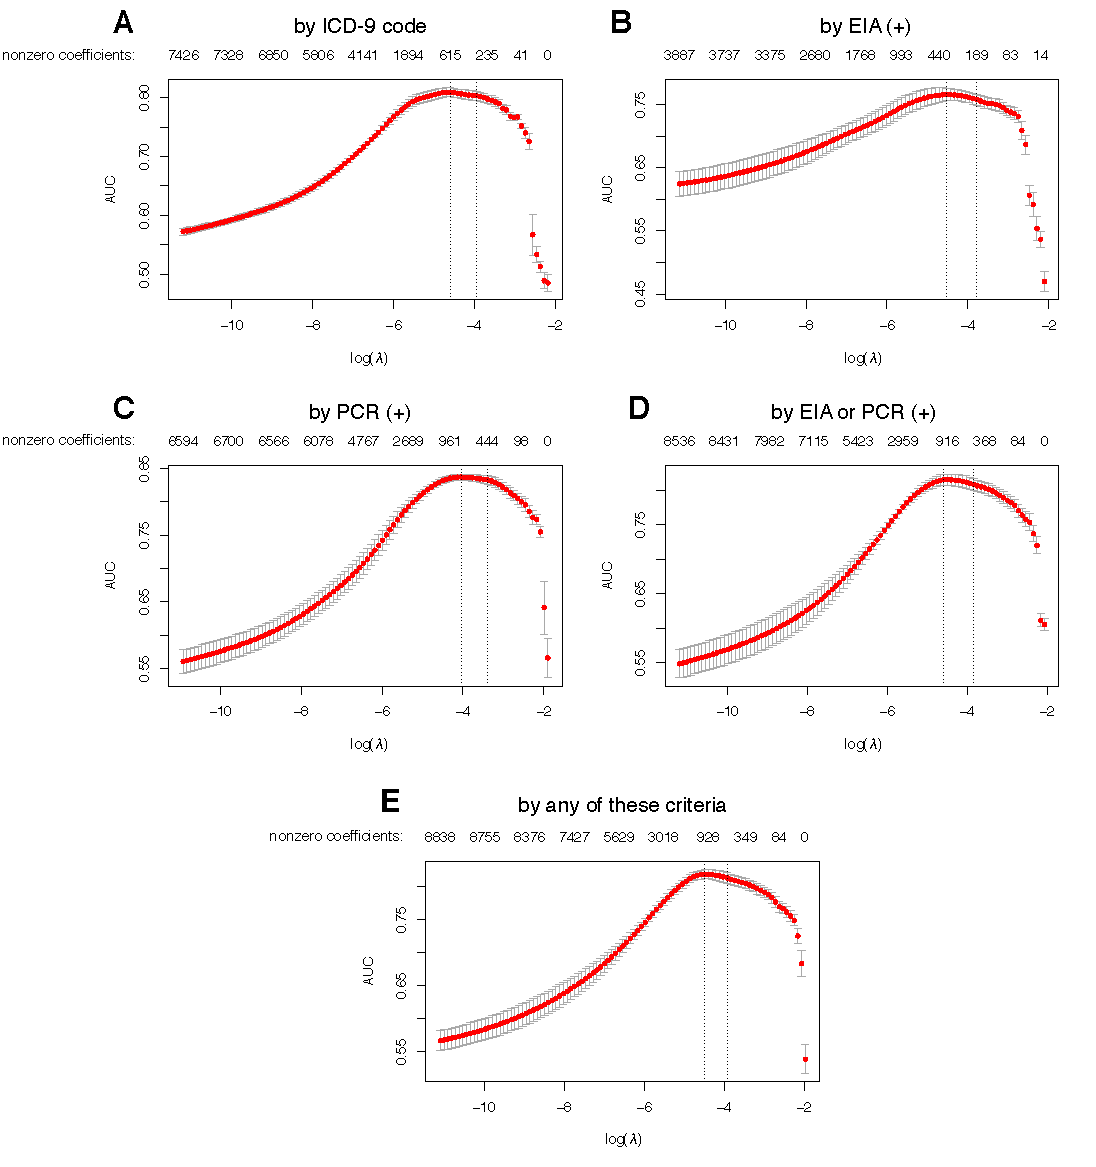
\includegraphics[width=0.9\textwidth]{chap5/S1_selecting_lambda}
  \fullwidthlabelcaption{fig:selecting_lambda}{Selection of the regularization penalty hyper-parameter $\lambda$}{
    \textbf{Empirical selection of the regularization penalty hyper-parameter $\lambda$.} A–E, mean area under the receiver operating characteristic curve (AUC) vs. $\log (\lambda)$ for each of the case definitions for \emph{C. difficile} infection, based on five-fold cross-validation. As the $\log (\lambda)$ penalty hyper-parameter increases, the number of variables left in the model (i.e., with nonzero coefficients) decreases; these are listed across the top of each plot. Vertical bars indicate standard errors. The $\log (\lambda)$ value with maximal mean AUC and the $\log (\lambda)$ value with mean AUC within 1 standard deviation of the maximum are highlighted by vertical dashed lines; the former was used for the final propensity models. ICD-9, International Classification of Diseases Ninth Revision; EIA, enzyme immunoassay; PCR, polymerase chain reaction.
  }
\end{figure*}
Nested cross validation while selecting $\lambda$ was used to evaluate AUROC (which are the performance values reported in Results), while the final propensity models were allowed to see the entire training dataset. 100 bootstrap resampling runs were used to estimate the 95\% AUROC confidence interval (CI). Since propensity models were intended to fairly assess risk at admission for CDI across both cases and controls, variables that could reflect workup or treatment of CDI (as opposed to pre-existing risk) were masked (Table \ref{tab:excluded_vars}). A board-certified infectious diseases physician reviewed the final set of variables selected by each model after regularization\footnote{FIXME: Include in an appendix?} to ensure that none of them reflected medical sequelae of CDI as opposed to potential risk factors.

Matching (1:1) on the propensity score was performed without replacement of controls using a nearest neighbor-matching algorithm and a caliper of 0.2 standard deviations of the logit of the propensity score,\autocite{Austin2011} after exact matching on gender and age divided into six ranges. To assess the performance of the matching, we calculated standardized mean differences\autocite{Austin2011} for age and gender, for which a difference between -0.1 and 0.1 is generally considered negligible,\autocite{Haukoos2015} and examined the distributions of the propensity scores between matched groups.

Furthermore, to ensure that propensity matching itself does not cause spurious changes in the outcome variable (LOS), we repeated the matching algorithm using the matched controls against remaining unmatched controls, creating a “matched-again” control cohort, with the expectation that re-matching controls should not, by itself, create significant differences in the outcome variable. For each case definition of CDI, differences of the median length of stay (LOS) between cases and matched controls were calculated and 95\% CIs were calculated from 10,000 bootstrap resampling runs. The minimum LOS was specified as 0.1 days (2.4 hours), with smaller values rounded up to this value. Statistical significance of differences in LOS was determined using two-sided Mann-Whitney \emph{U} tests. \emph{P} values for all contrasts reported in Figures 2 and 3 are conservatively Bonferroni-corrected for the full number of hypotheses (24). Kaplan-Meier plots were generated to examine the nonparametric maximum likelihood estimation for risk of discharge from the hospital between cases and matched controls, and 95\% CIs for these plots were derived from log-transformed standard errors.

To examine whether changes in LOS may have depended on the time of CDI onset, we repeated the above analysis for case definition (iv) stratified by the time of the first positive toxin assay result, using three ranges: 0–3 days, 3–8 days, and ≥8 days. Propensity models were again fitted to each of these case cohorts for matching as described previously, with the added condition that controls discharged before the start of the CDI time window were ineligible for matching, effectuating simplified balanced risk set matching.\autocite{Li2001} To assess matching performance, propensity score distributions for each group were examined once more, and LOS was analyzed similarly to the original five case definitions.

To further characterize dependence of LOS on the time of CDI onset, we fit a nonparametric multistate model consistent with previous studies.\autocite{Mitchell2014,Stevens2015,VanKleef2014} The model has two transient states (admitted-uninfected and admitted-infected) and one absorbing state (discharged); each patient starts in the admitted-uninfected state. Figure \ref{fig:etm_diagram} is a diagram of all allowed transitions. For all case definitions with a diagnosis time [(ii), (iii), and (iv)], an Aalen-Johansen estimator was used on the full, unmatched dataset to calculate time-varying hazards of each transition. Since the estimator is sensitive to regions with sparsity or outliers, the minimum LOS was specified as 1 day, the time of CDI diagnosis was left- or right-shifted to at least 0.5 days from admission and discharge events, and the model was computed to a precision of 0.1 day up to the 99th percentile LOS value [38.9, 41.9, and 40.9 days for case definitions (ii), (iii), and (iv), respectively]. The mean excess LOS was then estimated as the average difference in LOS between patients with and without CDI at each time t, weighted by the distribution of times spent in the uninfected state. Robust 95\% CIs were generated from 1,000 bootstrap resampling runs.

Analyses were performed in R 3.2.2 (R Foundation for Statistical Computing, Vienna, Austria) using the \texttt{glmnet},\autocite{Friedman2010} \texttt{ROCR},\autocite{Sing2005} \texttt{MatchIt},\autocite{Ho2011} \texttt{survival}, and \texttt{etm}\autocite{Allignol2011} packages. All software code for the analysis is available at: \url{https://github.com/powerpak/cdi-cost}

\section{Results}

371,622 records of visits during the study time range were queried from the EMR, with 23,968 variables extracted for each visit (Figure \ref{fig:exclusions}).
\begin{figure}[htb]
  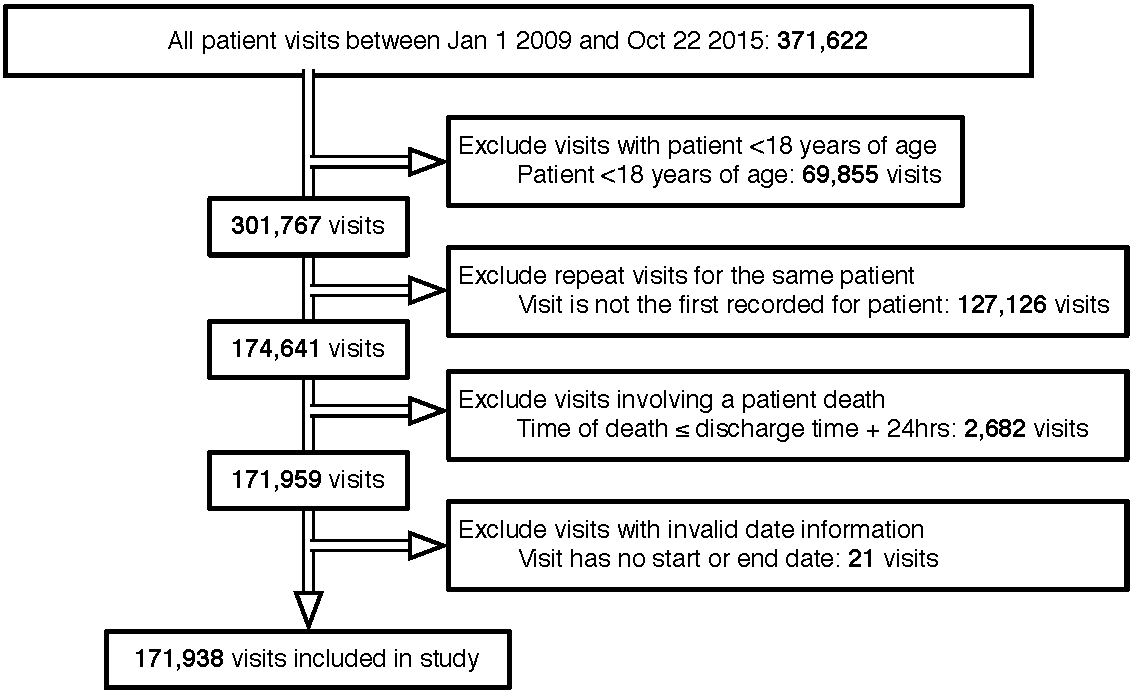
\includegraphics[width=\textwidth]{chap5/1b_methods_exclusion}               
  \caption[Inclusion/exclusion procedure for this study]{\textbf{Inclusion/exclusion procedure for the present study.} Double-line arrows indicate the procession of visit records.}
  \label{fig:exclusions}
\end{figure}
After filtering for the index visit per adult patient and excluding deaths and invalid dates, 171,938 visits were eligible for inclusion and classified into five overlapping case definitions for CDI. Case cohort sizes before matching and overlaps are depicted in Figure \ref{fig:set_intersections}.

\begin{marginfigure}[-4cm]
  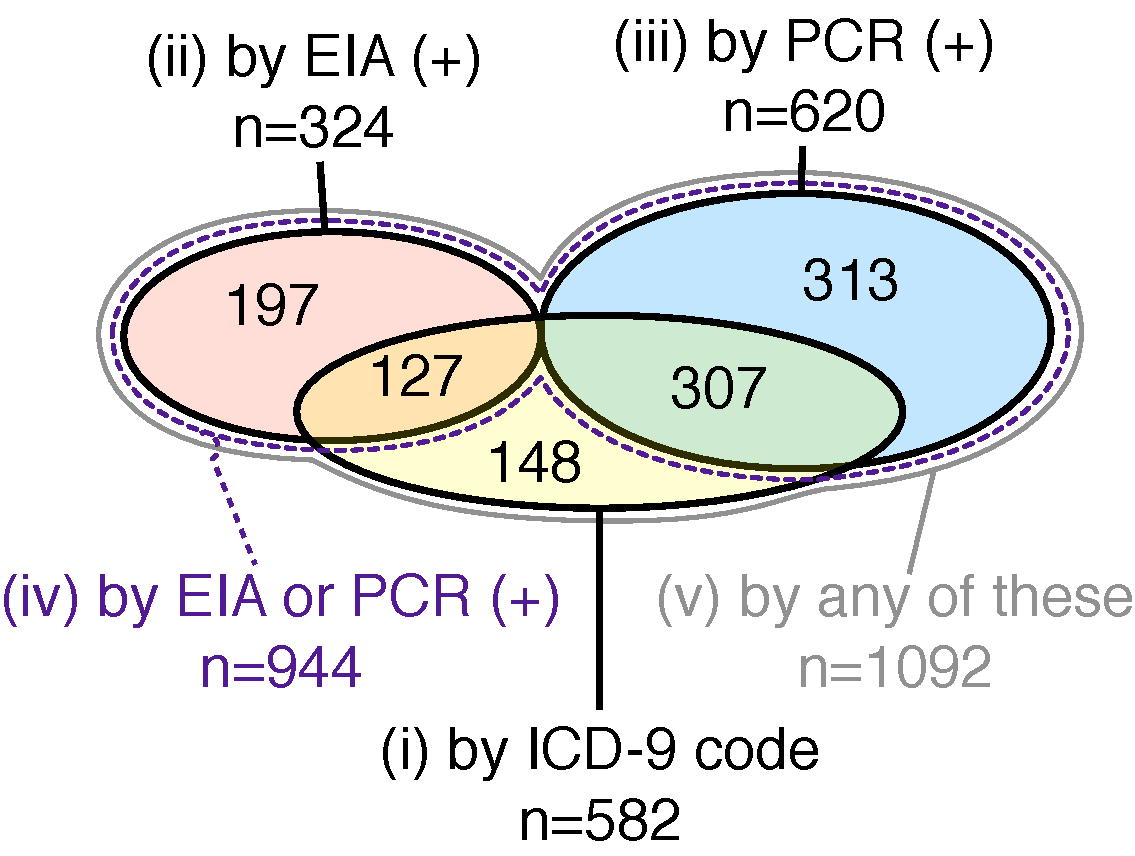
\includegraphics[width=\textwidth]{chap5/S2_set_intersections}               
  \caption[Cohort sizes for each case definition and cohort intersections before matching]{\textbf{Cohort sizes for each case definition and cohort intersections before matching.} Venn diagram of case cohort sizes for each of the five \emph{C. difficile} infection case definitions, before matching, with sizes of all intersections (overlaps) between case definitions. Areas are not to scale. There is no intersection between case definitions (ii) and (iii), since only the first positive toxin assay result for each visit was examined. Case definition (iv), “by EIA or PCR (+),” is a strict superset of case definitions (ii) and (iii). Case definition (v), “by any of these,” is a strict superset of case definitions (i), (ii), and (iii). Sizes of matched case cohorts are provided in Table FIXME.}
  \label{fig:set_intersections}
\end{marginfigure}

\begin{figure*}[tbp]
  \centering
  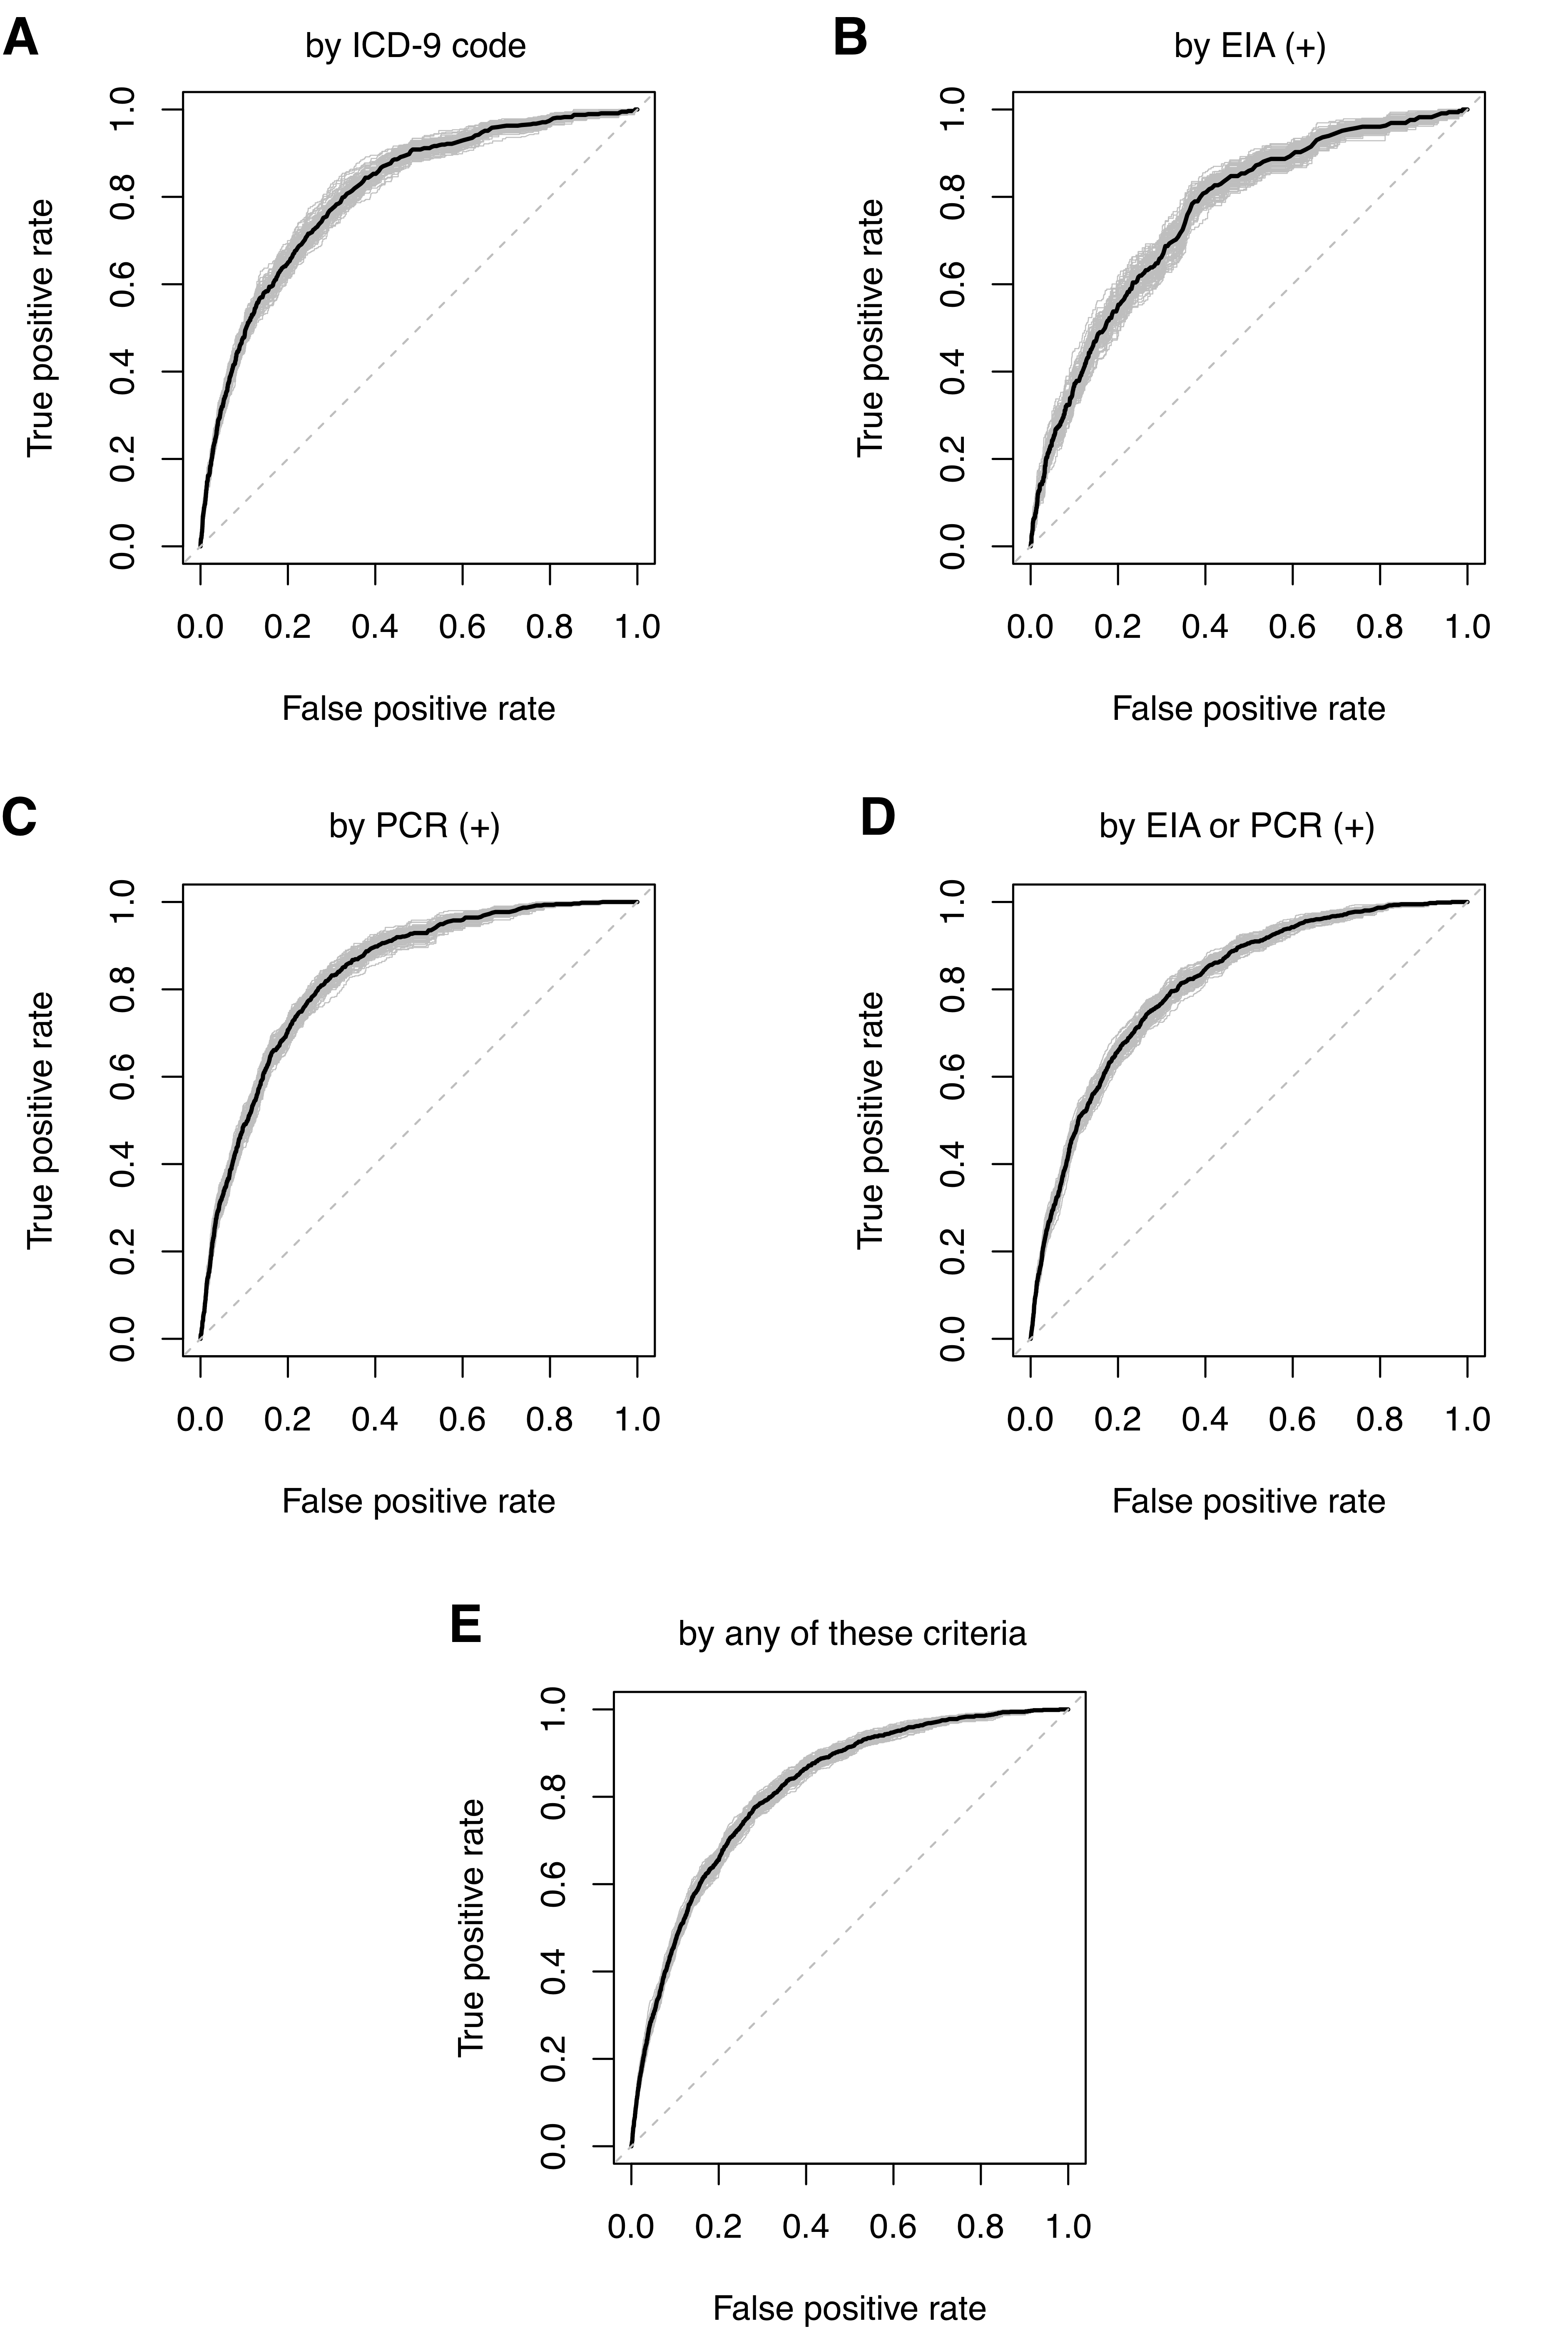
\includegraphics[width=0.7\textwidth]{chap5/S3_ROC}
  \fullwidthlabelcaption{fig:cdi_ROC}{Receiver operator characteristic curves for \emph{C. difficile} infection propensity models}{
    \textbf{Receiver operator characteristic curves for \emph{C. difficile} infection propensity models.} A-E, receiver operator characteristic (ROC) curve comparing the true positive rate against the false positive rate for every possible cutoff of the propensity score, for each of the five \emph{C. difficile} infection case definitions. ROCs are only measured on test data not used to train the models, under five-fold cross validation. Light grey lines indicate ROCs for 100 bootstrap samples. Area under each ROC is reported in the main text under Results. ICD-9, International Classification of Diseases Ninth Revision; EIA, enzyme immunoassay; PCR, polymerase chain reaction.
  }
\end{figure*}

Regularized logistic regression models predicting the risk of CDI acquisition were fit to EMR data from the first 24 hours of each admission for each case definition. The cross-validated mean area under the receiving operator characteristic (AUROC), measuring performance of each model, varied only slightly between case definitions (Figure \ref{fig:cdi_ROC}): (i) by ICD-9 code, 0.81 (95\% confidence interval [CI], 0.79–0.83); (ii) by positive toxin EIA, 0.76 (95\% CI, 0.74–0.78), (iii) by positive toxin PCR, 0.84 (95\% CI, 0.82–0.85), (iv) by either toxin assay, 0.81 (95\% CI, 0.80–0.82); (v) by any of these, 0.82 (95\% CI, 0.81–0.83). The number of selected variables in each model ranged from 373 to 1,027.

\begin{table*}[ht]
  \footnotesize
\begin{flushleft}%
\begin{tabular}{l P{3.15cm} P{1.6cm} P{1.6cm} P{1.2cm} P{1.6cm} P{1.6cm} P{1.2cm}}
  \toprule
  & & \multicolumn{6}{l}{\textbf{Matched cohorts for each CDI case definition}} \\
  \cmidrule(r){3-8}
  & & \multicolumn{3}{l}{(i) by ICD-9 code} & \multicolumn{3}{l}{(ii) by EIA (+)} \\
  \cmidrule(r){3-5}\cmidrule(r){6-8}
  & No. (\%) & \multicolumn{2}{l}{No. (\%)} & & \multicolumn{2}{l}{No. (\%)} & \\
  \cmidrule(r){2-2}\cmidrule(r){3-4}\cmidrule(r){6-7}
  \textbf{Characteristic} &
  All patients (n=171,936) &
  All controls (n=171,356) &
  Matched cases \& controls$^a$ (n=489) &
  SMD after matching (\emph{P} value) &
  All controls (n=73,647) &
  Matched cases \& controls$^a$ (n=274) &
  SMD after matching (\emph{P} value)
  \\
  \midrule
  Female sex & 101,964 (59) & 101,638 (59) & 278 (57) & 0 (1) & 44,132 (60) & 145 (53) & 0 (1) \\
  Age$^b$ \\
  \-\tabindent{}18-29 & 22,344 (13) & 22,266 (13) & 69 (14)   & \multirow{6}{1.5cm}{0.016 (0.86)} &
      9,552 (13) & 22 (8) & \multirow{6}{1.5cm}{0.018 (0.79)} \\
  \-\tabindent{}30-44 & 39,003 (23) & 38,898 (23) &  86 (18)  &  & 16,451 (22) & 26 (9)  & \\
  \-\tabindent{}45-59 & 37,234 (22) & 37,129 (22) &  90 (18)  &  & 15,956 (22) & 58 (21) & \\
  \-\tabindent{}60-74 & 43,946 (26) & 43,802 (26) & 122 (25)  &  & 18,407 (25) & 83 (30) & \\
  \-\tabindent{}75-90 & 26,167 (15) & 26,041 (15) & 106 (22)  &  & 11,817 (16) & 70 (26) & \\
  \-\tabindent{}≥90   &  3,244 (2)  &  3,220 (2)  &  16 (3)   &  &  1,464 (2)  & 15 (5)  & \\
  \bottomrule
\end{tabular}

\vspace{1em}

\begin{tabular}{l P{1.3cm} P{1.2cm} P{1.2cm} P{1.3cm} P{1.2cm} P{1.2cm} P{1.3cm} P{1.2cm} P{1.2cm}}
  \toprule
  & \multicolumn{6}{l}{\textbf{Matched cohorts for each CDI case definition (cont.)}} \\
  \cmidrule(r){2-10}
  & \multicolumn{3}{l}{(iii) by PCR (+)} & \multicolumn{3}{l}{(iv) by EIA or PCR (+)} & 
    \multicolumn{3}{l}{(v) by any of the criteria} \\
  \cmidrule(r){2-4}\cmidrule(r){5-7}\cmidrule(r){8-10}
  & \multicolumn{2}{l}{No. (\%)} & & \multicolumn{2}{l}{No. (\%)} & & \multicolumn{2}{l}{No. (\%)} & \\
  \cmidrule(r){2-3}\cmidrule(r){5-6}\cmidrule(r){8-9}
  \textbf{Characteristic} &
  All controls (n=97,351) &
  Matched cases \& controls$^a$ (n=493) &
  SMD after matching (\emph{P} value) &
  All controls (n=170,994) &
  Matched cases \& controls$^a$ (n=788) &
  SMD after matching (\emph{P} value) &
  All controls (n=170,846) &
  Matched cases \& controls$^a$ (n=945) &
  SMD after matching (\emph{P} value)
  \\
  \midrule
  Female sex & 57,340 (59) & 254 (52) & 0 (1) & 101,469 (59) & 408 (52) & 0 (1) & 101,390 (59) & 493 (52) & 0 (1) \\
  Age$^b$ \\
  \-\tabindent{}18-29 & 12,714 (13) &  47 (10) & \multirow{6}{1.2cm}{0.005 (0.99)} & 
      22,265 (13) & 79 (9) & \multirow{6}{1.2cm}{0.003 (0.98)} &
      22,245 (13) & 87 (9) & \multirow{6}{1.2cm}{0.004 (0.93)} \\
  \-\tabindent{}30-44 & 22,430 (23) &  72 (15) &  & 38,879 (23) & 124 (13) & & 38,845 (23) & 134 (14) & \\
  \-\tabindent{}45-59 & 21,069 (22) & 117 (24) &  & 37,025 (22) & 209 (23) & & 36,999 (22) & 208 (22) & \\
  \-\tabindent{}60-74 & 25,273 (26) & 136 (28) &  & 43,680 (26) & 266 (29) & & 43,643 (26) & 267 (28) & \\
  \-\tabindent{}75-90 & 14,120 (15) & 114 (23) &  & 25,936 (15) & 231 (24) & & 25,912 (15) & 217 (23) & \\
  \-\tabindent{}≥90   &  1,745 (2)  &   7 (1)  &  &  3,209 (2)  &  35 (3)  & &  3,202 (2)  &  32 (3)  & \\
  \bottomrule
\end{tabular}
\end{flushleft}
  \caption[Demographic characteristics of the study population and matched cohorts]{\textbf{Demographic characteristics of the study population and matched cohorts.} Abbreviation: CDI, Clostridium difficile infection; ICD-9, International Classification of Diseases Ninth Revision; EIA, enzyme immunoassay; PCR, polymerase chain reaction; SMD, standardized mean difference. $^a$Separate columns are unnecessary because 1:1 exact matching was performed on the characteristics shown, and therefore all values are identical. $^b$SMD is shown for age treated as a continuous variable; coarsened exact matching was performed using the listed age ranges.
}
  \label{tab:cdi_pts}
\end{table*}

For each case definition, over 75\% of cases were successfully matched by propensity score to controls (Figure \ref{fig:set_intersections} and Table \ref{tab:cdi_pts}). The groups are well matched on demographics and propensity scores (all \emph{P} values >0.1 and standardized differences between –0.1 and 0.1; propensity score distributions in Figure \ref{fig:psm_density}).
\begin{figure}[htb]
  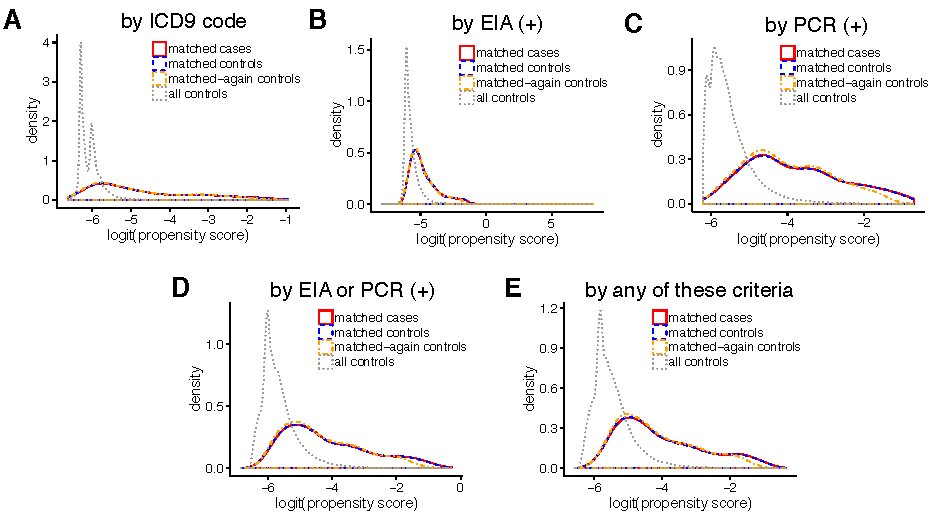
\includegraphics[width=\textwidth]{chap5/S4_psm_density}
  \caption[Propensity score distributions for matched cohorts for each \emph{C. difficile} infection case definition]{
    \textbf{Propensity score distributions for matched cohorts for each \emph{C. difficile} infection case definition.} A-E, density plots of propensity score distributions for matched cases, matched controls, matched-again controls, and all controls for each of the five CDI case definitions. Matched-again controls are derived from a second round of matching between the case-matched controls from the first round of matching and remaining unmatched controls. All X axes are logit-scaled. All Y axes are scaled to unit probabilities; the area under every curve equals 1. The matching algorithm intends to align the propensity score distributions for all of the matched groups.
  }
  \label{fig:psm_density}
\end{figure}
Differences in the median LOS between matched case and control cohorts for all CDI case definitions were strongly statistically significant, although the magnitude of the differences varied greatly between definitions (Figure \ref{fig:violin}). The differences in the median LOS by case definition were: (i) by ICD-9 code, 3.1 days (95\% CI, 2.2–3.9); (ii) by positive toxin EIA, 10.1 days (95\% CI, 7.3–12.2), (iii) by positive toxin PCR, 6.6 days (95\% CI, 5.0–8.1), (iv) by either toxin assay, 7.2 days (95\% CI, 5.8–8.3); and (v) by any of these, 5.7 days (95\% CI, 4.5–6.6). 
\begin{figure}[htb]
  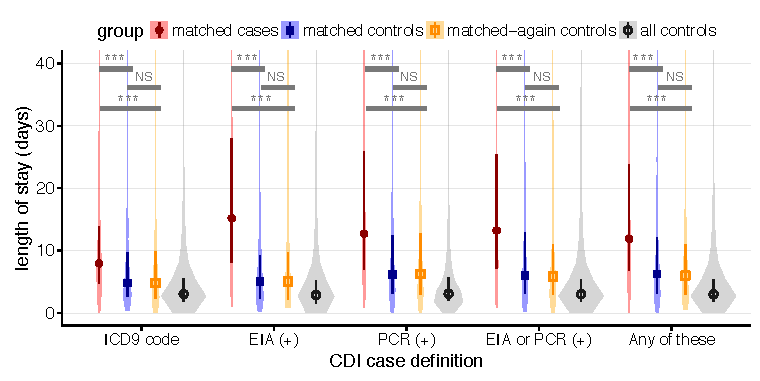
\includegraphics[width=\textwidth]{chap5/2a_violin}
  \caption[Changes in length of stay for five case definitions of \emph{C. difficile} infection, not accounting for time of infection]{
    \textbf{Changes in length of stay for five case definitions of \emph{C. difficile} infection, not accounting for time of infection.} Violin plots of the distributions in length of stay for matched cases, matched controls, matched-again controls, and all controls, for each of the five case definitions. Darker points and vertical bars depict the median and interquartile range for each group. Horizontal bars depict Mann-Whitney \emph{U} tests for significance of differences between groups (***, Bonferroni-corrected \emph{P} < 0.001; NS, not significant [\emph{P} > 0.1]). CDI, \emph{C. difficile} infection.
  }
  \label{fig:violin}
\end{figure}
There were no significant differences in LOS for a second round of matching between matched controls and remaining controls (matched-again controls) for any of the case definitions (Figure \ref{fig:violin}). Kaplan-Meier curves for the time-dependent risk of being discharged from the hospital showed significant differences between matched case and control cohorts up to post-admit day 60 for all case definitions except ICD-9 code (Figure \ref{fig:survival}).

\begin{figure}[htb]
  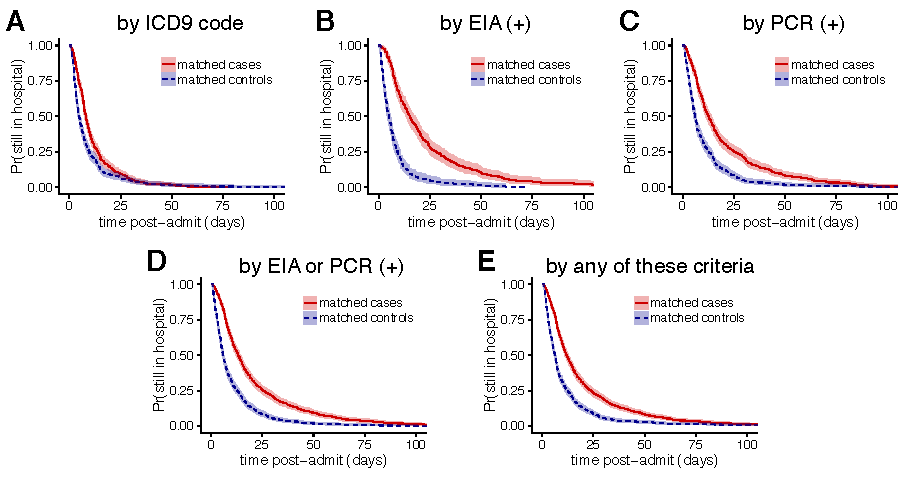
\includegraphics[width=\textwidth]{chap5/2b_survival}
  \caption[Kaplan-Meier plots for length of stay, not accounting for time of infection]{
    \textbf{Kaplan-Meier plots of the time-dependent probability for a patient to still be in the hospital, not accounting for time of infection.} A-E, Kaplan-Meier plots of the time-dependent probability for a patient to still be in the hospital, comparing matched cases and controls for each case definition of \emph{C. difficile} infection. Shaded areas depict 95\% confidence intervals calculated from standard errors. ICD9, International Classification of Diseases Ninth Revision; EIA, enzyme immunoassay; PCR, polymerase chain reaction.
  }
  \label{fig:survival}
\end{figure}

Estimates of LOS associated with CDI are inflated by dependencies on time-to-infection—if longer pre-infection LOS increases CDI risk, i.e., reverse causation, this leads to overestimates in attributable cost.\autocite{Mitchell2014,Stevens2015} We therefore performed two follow-up analyses to account for this. First, we stratified the LOS comparison by the time of CDI diagnosis for case definition (iv) into 0–3 day, 3–8 day, and ≥8 day case cohorts, training new propensity models for another matched comparison, with similar matching performance (Figure \ref{fig:timedep_psm_density}).
\begin{figure}[htb]
  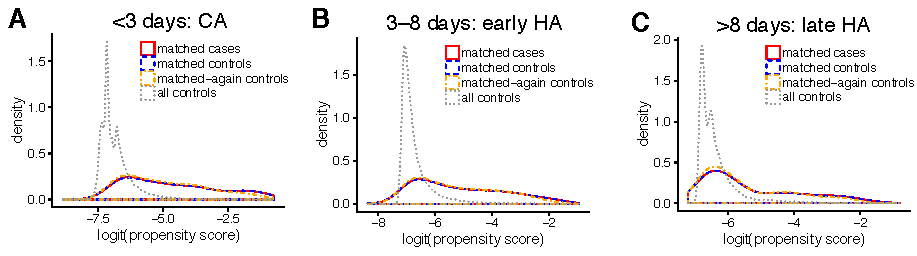
\includegraphics[width=\textwidth]{chap5/S5_timedep_psm_density}
  \caption[Propensity score distributions for matched cohorts stratified by time of \emph{C. difficile} infection diagnosis][-1.5cm]{
    \textbf{Propensity score distributions for matched cohorts stratified by time of CDI diagnosis.} A-C, density plots of propensity score distributions for matched cases, matched controls, matched-again controls, and all controls for cases defined by any positive toxin assay, stratified by the time to infection. Matched-again controls are derived from a second round of matching between the case-matched controls from the first round of matching and remaining unmatched controls. All X axes are logit-scaled. All Y axes are scaled to unit probabilities; the area under every curve equals 1. The matching algorithm intends to align the propensity score distributions for all of the matched groups. CA, community acquired; HA, health- care associated.
  }
  \label{fig:timedep_psm_density}
\end{figure}
Since 3 days (or 72 hours) is a typical cutoff for differentiating community acquired (CA) from healthcare-associated (HA) CDI,\autocite{Longtin2016,Polage2015} these strata were named “CA,” “early HA,” and “late HA,” respectively. As suspected, stratification revealed a positive correlation between time of diagnosis and the CDI-associated difference in LOS (Figure \ref{fig:timedep_violin}). The differences in medians were: for CA, 2.5 days (95\% CI, 1.2–3.4); early HA, 3.1 days (95\% CI, 1.8–4.4); and late HA, 14.0 days (95\% CI, 9.9–17.1). All comparisons between matched cases and controls were again strongly statistically significant, and comparisons between matched controls and matched-again controls were not significant (Figure \ref{fig:timedep_violin}). Kaplan-Meier plots likewise confirmed a correlation between time of CDI diagnosis and the difference in time-dependent discharge risk (Figure \ref{fig:timedep_survival}).

\begin{figure}[htb]
  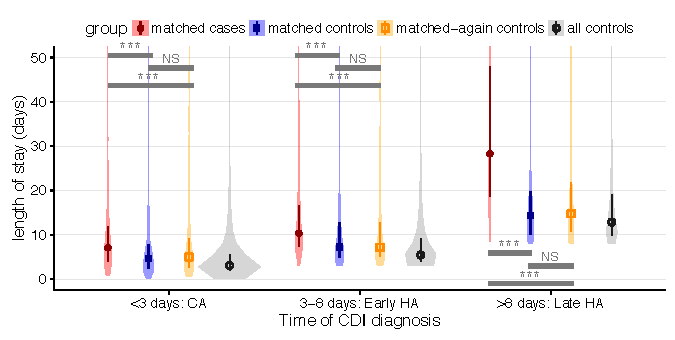
\includegraphics[width=\textwidth]{chap5/3a_timedep_violin}
  \caption[Changes in length of stay for \emph{C. difficile} infection defined by any positive toxin assay and stratified by the time to infection]{
    \textbf{Changes in length of stay for \emph{C. difficile} infection defined by any positive toxin assay, stratified by the time to infection.} Violin plots of the distributions in length of stay for matched cases, matched controls, matched-again controls, and all controls, for three ranges of the result time for the first positive toxin assay. Points and vertical bars depict the median and interquartile range for each group. Horizontal bars depict Mann-Whitney \emph{U} tests for significance of differences between groups (***, Bonferroni-corrected \emph{P} < 0.001; NS, not significant [P > 0.1]). CA, community acquired; HA, healthcare associated.
  }
  \label{fig:timedep_violin}
\end{figure}
\begin{figure}[htb]
  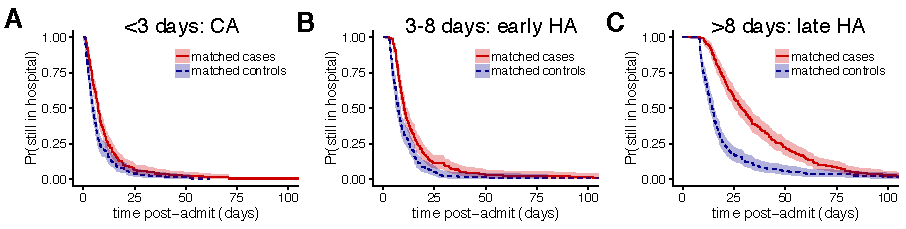
\includegraphics[width=\textwidth]{chap5/3b_timedep_survival}
  \caption[Kaplan-Meier plots for length of stay, stratifying patients by the time to infection]{\textbf{Kaplan-Meier plots of the time-dependent probability for a patient to still be in the hospital, stratifying patients by the time to infection.} A-C, comparison of matched \emph{C. difficile} infection cases and controls for the same three ranges of the time of the first positive toxin assay, stratified by the time to infection. Shaded areas depict 95\% confidence intervals calculated from standard errors. CA, community acquired; HA, healthcare associated.
  }
  \label{fig:timedep_survival}
\end{figure}

To further address reverse causation, we fit a multistate model similar to previously published studies\autocite{Mitchell2014,Stevens2015,VanKleef2014} that explicitly estimates time-dependent, competing risks of transitioning to a CDI-positive state vs. being discharged. Figure \ref{fig:etm_diagram} depicts the three states and allowed transitions of the model. After fitting the model for the case definitions with a time of diagnosis (ii, iii, and iv), the expected remaining LOS can be compared across cohorts that have already transitioned to the CDI infected state vs. those that are still CDI negative at any given timepoint (Figure \ref{fig:etm}).
\begin{marginfigure}
  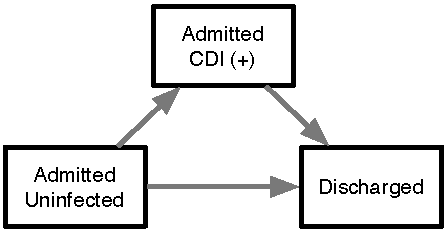
\includegraphics[width=\textwidth]{chap5/4a_etm_diagram}               
  \caption[Multistate model of \emph{C. difficile} infection]{\textbf{Multistate model of \emph{C. difficile} infection.} Three states of the multistate model and allowed transitions. Patients may only transition in the direction of the arrows.}
  \label{fig:etm_diagram}
\end{marginfigure}
To summarize the overall relationship between CDI and LOS, differences in LOS were weighted by the distribution of times spent in the initial state and averaged. The average differences for each case definition were: (ii) by positive toxin EIA, 3.0 days (95\% CI, 2.0–4.0); (iii) by positive toxin PCR, 3.5 days (95\% CI, 2.7–4.5); and (iv) by either toxin assay, 3.3 days (95\% CI, 2.6–4.0). Notably, the 95\% CI for the difference in cohort (iv) overlaps the 3.1 day difference for the “early HA” stratum of the propensity-matched analysis in the same cohort.

\begin{figure*}[htb]
  \centering
  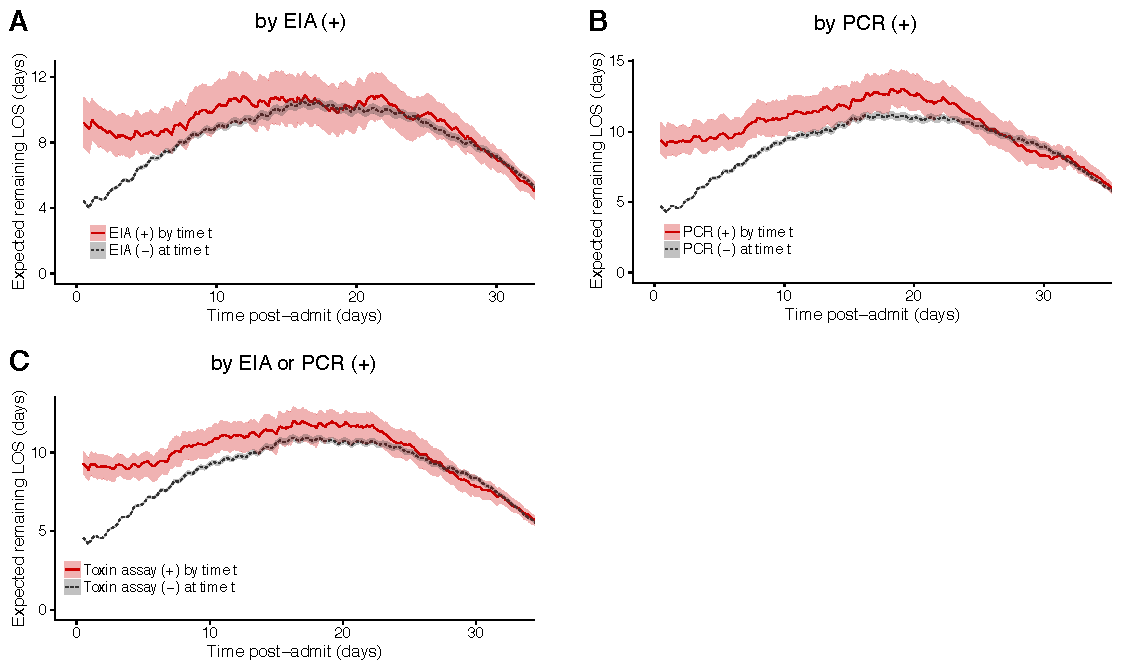
\includegraphics[width=0.8\textwidth]{chap5/4b_etm}
  \caption[Expected remaining length of stay for \emph{C. difficile} infection case definitions as predicted by a multistate model][-4cm]{\textbf{Expected remaining length of stay for \emph{C. difficile} infection case definitions predicted by a multistate model.} A-C, expected remaining LOS for each post-admit time $t$ depending on whether the patient has had a positive (+) toxin assay by that timepoint, for each of the case definitions involving toxin assays. Shaded areas depict 95\% confidence intervals calculated from 1,000 bootstrap samples. CDI, Clostridium difficile infection; EIA, enzyme immunoassay; PCR, polymerase chain reaction; LOS, length of stay.
  }
  \label{fig:etm}
\end{figure*}

\section{Discussion}

This study examined nearly seven years of uncurated EMR data for a single hospital and determined associated costs of CDI as defined by either visit diagnosis codes or lab results. In the analysis unadjusted for time-to-infection, differences in LOS were often greater than national averages from similar unadjusted studies,\autocite{Gabriel2014,Zhang2016,Zimlichman2013} but changes in the case definition resulted in substantial changes in the estimated differences in LOS. Although two hospitals reported good concordance between ICD-9 codes and CDI toxin assay results,\autocite{Dubberke2006,Scheurer2007} this is not necessarily the case for all hospitals. We found that 75\% of ICD-9 coded visits involved a positive toxin assay, while only 46\% of visits with a positive toxin assay had the ICD-9 code (Figure \ref{fig:set_intersections}). Changes in LOS were not significantly different between EIA and PCR toxin assays, although our study was limited by a smaller sample size for EIA (+) cases. Toxin assays are likely a more reliable CDI definition given their basis in clinical symptoms and evidence for CDI, whereas medical coding suffers from biases introduced by billing and reimbursement.\autocite{Rhee2015,Romano1994}

Treating CDI as a baseline condition by ignoring the relationship between pre-infection hospital exposure and CDI risk overestimates associated costs.\autocite{Graves2010,Mitchell2014,Stevens2015} Unlike visit diagnosis codes, toxin assay results provide a presumptive time-to-infection that we incorporated into two different statistical methods addressing time-dependent bias. When using a case definition of either toxin assay being positive, the measured difference in LOS in the multistate model corresponded closely with the difference seen in the “early HA” stratum of a time-stratified propensity-matched analysis (3.3 vs.\ 3.1 days). This suggests that measured differences in this study robustly reflect associated costs of HA-CDI in our patient population. Since estimates for each time-to-infection stratum in the matching analysis differed greatly (Figure \ref{fig:timedep_violin}–\ref{fig:timedep_survival}), time-to-infection clearly contributed bias to the unstratified analysis (Figure \ref{fig:violin}–\ref{fig:survival}), demonstrating how the many studies that ignore this bias\autocite{Gabriel2014,Zhang2016,Zimlichman2013} produce inflated estimates. In our dataset, ignoring time-dependent bias would lead to a more than two-fold overestimation of CDI-associated LOS. Given our findings, we cautiously interpret the results of meta-analyses that conflate ICD-9 code and toxin assay case definitions and often ignore time-dependent bias.\autocite{Gabriel2014,Ghantoji2010,Zhang2016}  

To our knowledge, this is the first study that uses machine learning on uncurated EMR data to estimate the local cost of CDI. Our models of CDI risk performed on par with prior models fitted to lower-dimensional data.\autocite{Dubberke2011,Tanner2009,Wiens2014} Since our models are based on tens of thousands of structured fields in the EMR that require neither chart review nor manual curation beyond masking known CDI-related effects, re-analysis of future data is inexpensive. Starting from exported visit data, the entire analysis runs in several hours on standard desktop computers. Therefore, the effects of new interventions against CDI can be efficiently monitored over time, e.g., continually testing whether new treatments actually lower the CDI-associated LOS or quantifying cost savings of new preventive strategies that decrease CDI incidence. Changes in LOS can be extrapolated to approximate economic costs by multiplying by the average cost of extra inpatient-days as LOS is the main contributor to CDI’s cost.\autocite{Graves2010,McGlone2012,Wilcox1996,Zimlichman2013} In our dataset, using the time-dependency adjusted differences in LOS of 3.1–3.3 days and the national average cost of additional inpatient-days for CDI cases,\autocite{Zimlichman2013} the median cost associated with each case would be approximately \$10,600–11,300; this is substantial in comparison to the national average price for an inpatient visit—approximately \$13,000 in 2011.\autocite{Cooper2015} Using the average yearly caseload observed in the dataset for toxin assay positive cases, our figures represent an annual accounting cost to Mount Sinai of approximately \$1.5 million, not including the opportunity cost of bed occupancy by CDI patients or the impact on infection control resources.\autocite{Graves2010} In principle, our analysis is generalizable to any HAI where lab results recorded in the EMR robustly reflect the incidence of infections.

Our study has several limitations. The analysis was designed with conservative assumptions, preferring that the models underestimate rather than overestimate changes associated with CDI. For example, restricting to one index visit per patient certainly excluded many repeat visits for recurrent CDI, which are known to incur higher costs.\autocite{Dubberke2008,Dubberke2014,Rodrigues2016} We preferred a relatively simple machine learning technique, elastic net regularized generalized linear models, because of its transparency in variable selection and unparalleled speed on sparse training data. More advanced techniques might marginally improve propensity model accuracy at the expense of computational complexity and model interpretability. EMR data has known drawbacks compared to clinical research data, such as limitations in time precision, the sparsity of the data, and increased opportunity for coding error. Also, retrospective matching-based studies face known trade-offs in estimating actual effects of HAIs,\autocite{Graves2010} so we used two separate statistical approaches to control for time-dependent bias, ultimately finding congruous results. We did not have structured billing data, so we cannot trace itemized costs and characterize the exact relationship between LOS and costs beyond the proportional estimate above. Finally, only one hospital’s data was used to implement this analysis, which would benefit from comparison to other hospitals’ data. Therefore, we provide complete code for our analysis so that it may be re-implemented elsewhere and improved by the community.

\section{Conclusions}

\newthought{Two independent} statistical analyses adjusting for time-dependent bias produced similar results for the CDI-associated change in LOS at Mount Sinai (3.1 and 3.3 days), suggesting that automated methods based on machine learning and uncurated EMR data robustly and conservatively estimate the local cost of an HAI in both LOS and financial terms. This procedure is transparent, reproducible, and inexpensive, suggesting that hospitalists and infection control officers can leverage EMR data to estimate their specific, local costs of HAIs on an ongoing basis rather than relying on widely varying benchmarks published by other institutions.

\section*{Notes}

\subsection*{Contributors}

Theodore Pak (\smallcaps{TRP}), Kieran Chacko (\smallcaps{KC}), Timothy O'Donnell (\smallcaps{TO}), Shirish Huprikar (\smallcaps{SH}), Harm van Bakel (\smallcaps{HVB}), Andrew Kasarskis (\smallcaps{AK}), and Erick R. Scott (\smallcaps{ERS}) contributed to this study. \smallcaps{TRP}, \smallcaps{KC}, \smallcaps{AK}, and \smallcaps{ERS} designed the study and developed the models. \smallcaps{TRP}, \smallcaps{KC}, \smallcaps{TO}, \smallcaps{SH}, \smallcaps{HVB}, \smallcaps{AK}, and \smallcaps{ERS} acquired the data. \smallcaps{TRP} performed the data analysis and created all figures in this chapter. \smallcaps{SH} reviewed selected variables for the propensity model. \smallcaps{TO} provided technical support, and \smallcaps{HVB}, \smallcaps{SH}, and \smallcaps{AK} provided administrative and material support. \smallcaps{AK} and \smallcaps{ERS} supervised the study. \smallcaps{TRP} wrote the first draft of this chapter. \smallcaps{TRP} is the first author on the corresponding submitted manuscript.

\subsection*{Funding}

This work was supported by the Icahn Institute for Genomics and Multiscale Biology at Mount Sinai, and also in part by the NIH/NIAID grants F30-AI122673 (\smallcaps{TRP}), T32-GM007280 (\smallcaps{TRP}), and R01-AI119145 (\smallcaps{HVB}, \smallcaps{KC}).

\subsection*{Conflict of Interest}

The authors have no conflicts of interest to disclose.

\subsection*{Acknowledgements}

This work was supported in part by the resources and expertise of the Department of Scientific Computing at the Icahn School of Medicine at Mount Sinai. We thank Deena Altman, Camille Hamula, and Gopi Patel for their assistance in improving the design of the study and reviewing the manuscript.